\documentclass[runningheads]{llncs}

\usepackage[T1]{fontenc}

%\DeclareMathAlphabet{\mathcal}{OMS}{cmsy}{m}{n}
\DeclareSymbolFont{letters}{OML}{txmi}{m}{it} % Redefines Greek

\usepackage{microtype}
\usepackage{mathtools}
\usepackage{amsmath,amssymb,amsfonts}
\usepackage{wasysym}
\usepackage{tikz}
\usepackage{xspace}
\usepackage{enumerate}
\usepackage{algorithm}
\usepackage{algorithmicx}
\usepackage{prftree}
\usepackage[noend]{algpseudocode}
\usepackage{subcaption}
\usepackage{multirow}
\usepackage{adjustbox}
\usepackage{paralist}
\usepackage{url}
\usepackage{cite}
\usepackage{listings}
\usetikzlibrary{automata}

\graphicspath{{icons/}}
\usepackage[hidelinks]{hyperref}

\makeatletter
\def\@citecolor{blue}%
\def\@urlcolor{blue}%
\def\@linkcolor{blue}%
\def\UrlFont{\rmfamily}

%\def\orcidID#1{\relax{\href{https://orcid.org/#1}{\protect\raisebox{-1.25pt}{\protect\includegraphics{ORCID_Color.eps}}}}}
\makeatother

%\newtheorem{definition}{Definition}
%\newtheorem{proposition}[definition]{Proposition}
%\newtheorem{conjecture}[definition]{Conjecture}
\newcommand{\Lex}{\texttt{Lex}}
\newcommand{\kw}[1]{{\color{purple}\texttt{#1}}}

\linepenalty=1000

\begin{document}

\title{Lex: A Programming Language for Developing Enforceable Legal Formalizations}

\author{Jonas Degelo \and François Hublet \and Jakob Merane}

\authorrunning{J. Degelo et al.}

\institute{ETH Zürich, Switzerland\\\email{\{degeloj,fhublet,jmerane\}@ethz.ch}}

\maketitle

%\vspace*{-2ex}
\begin{abstract}
  \keywords{Legal formalization \and Programming languages.}
\end{abstract}
%

%
\section{Introduction}

\section{Syntax}

\subsection{Types}

\Lex{} has four base types: \kw{int} (integers), \kw{float} (floating-point numbers), \kw{bool} (booleans), and \kw{str} (strings).
New types can be declared as follows:
\begin{align*}
  type\_decl &::= \kw{type}~ident~[[\kw{is}|\kw{subtype}]~ident]
\end{align*}
When another, alreadly existing type name is specified after the \kw{is} keyword, the newly declared type is created as a copy of that existing type. As a consequence, the new type will have the same internal representation and take the same values as the existing type. However, the existing type and the new type will still be considered distinct types by \Lex{}'s type system (see example below). In contrast, the \kw{subtype} keyword support specifying a new type as a subtype of an existing type. In this case, the new type will have both the same internal representation and the capacity to be used in any context where the existing type could be used.

\begin{example}
  Consider the following declarations:
  \begin{align*}
    &\kw{type}~\texttt{id}~\kw{is}~\kw{string}\\
    &\kw{type}~\texttt{user\_id}~\kw{subtype}~\texttt{id}
  \end{align*}
  Further, consider an event with signature
  $\texttt{A}(\texttt{b}\kw{:}\texttt{id}, \texttt{c}\kw{:}\kw{string})$
  and a variable \texttt{uid} of type \texttt{user\_id}. The expression
  $\texttt{A}(\texttt{uid},\kw{"foo"})$ is type-correct, since \texttt{user\_id}
  is a subtype of \texttt{id}. The expression $\texttt{A}(\texttt{uid},\texttt{uid})$ is
  not type-correct, since \texttt{user\_id} is not a subtype of \kw{string}
  (because \texttt{id} is not a subtype of \kw{string}). On the other hand,
  $\texttt{A}(\kw{"foo"},\kw{"foo"})$ is type-correct since the type \texttt{id} can
  contain string values.
\end{example}

\subsection{Events}

The syntax for event declarations is as follows:
\begin{align*}
  capabilities ::=&~\kw{observable} \mid \kw{suppressable} \mid \kw{causable} \mid \kw{internal}\\
                &\mid \kw{observable}~\kw{causable} \mid \kw{causable}~\kw{observable} \\
                &\mid \kw{suppressable}~\kw{causable} \mid \kw{causable}~\kw{suppressable} \\
  event\_decl ::=&~ capabilities~\kw{event}~ident~ \\
                &~ [\kw{"""}event\_desc\kw{"""}]\\
                 &\qquad ident_{11}~\kw{:}~ident_{12}\\
                 &\qquad \dots\\
                 &\qquad ident_{k1}~\kw{:}~ident_{k2}
\end{align*}
where $event\_desc$ is a string that can contain special placeholders $\kw{\{}ident_{i1}\kw{\}}$
for $1 \leq i \leq k$. The capabilities associated to an event are organized into the following lattice, where $a \rightarrow b$ denotes that $a$ is strictly weaker than $b$.
\begin{figure}
  \centering
  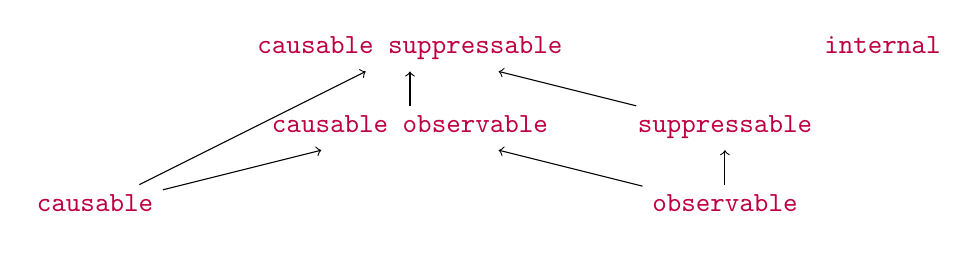
\begin{tikzpicture}
    \node[text depth=0.1cm] (cau_sup) at (0,0) {\kw{causable suppressable}};
    \node[text depth=0.1cm] (cau_obs) at (0,-1) {\kw{causable observable}};
    \node[text depth=0.1cm] (cau) at (-4,-2) {\kw{causable}};
    \node[text depth=0.1cm] (sup) at (4,-1) {\kw{suppressable}};
    \node[text depth=0.1cm] (obs) at (4,-2) {\kw{observable}};
    \node[text depth=0.1cm] (int) at (6,0) {\kw{internal}};
    \draw[->] (cau) -- (cau_sup);
    \draw[->] (sup) -- (cau_sup);
    \draw[->] (obs) -- (sup);
    \draw[->] (cau_obs) -- (cau_sup);
    \draw[->] (cau) -- (cau_obs);
    \draw[->] (obs) -- (cau_obs);
  \end{tikzpicture}
  \caption{Capability lattice}
\end{figure}

The pairs of identifiers $ident_{i1}\kw{:} ident_{i2}$ contained in the event declaration determine an (ordered) list of event parameters ($ident_{i1}$) and their types ($ident_{i2}$). Finally, the event description $event\_desc$ provides the high-level semantics of the event, which should refer to the parameters $ident_{i1},\dots,ident_{k1}$ using the $\kw{\{} ident_{i1}\kw{\}}$ syntax.
\begin{example}
  The following code declares a new suppressable event capturing personal data processing in a system, assuming three previously defined types \texttt{processing\_id}, \texttt{processor\_id}, and \texttt{data\_id}.
  \begin{align*}
    &\kw{suppressable}~\kw{event}~\texttt{PersonalDataProcessing}\\
    &\kw{"""}\\
    &\text{\itshape processor \kw{\{}x\kw{\}} is processing personal data \kw{\{}z\kw{\}} as part}\\
    &\text{\itshape of processing operation \kw{\{}ep\kw{\}}}\\
    &\kw{"""}\\
    &\qquad\begin{array}{lll}
             \texttt{ep}&\kw{:}&\texttt{processing\_id}\\
             \texttt{x}&\kw{:}&\texttt{processor\_id}\\
             \texttt{z}&\kw{:}&\texttt{data\_id}
           \end{array}
  \end{align*}
\end{example}

\end{document}
%%% Local Variables:
%%% mode: latex
%%% TeX-master: t
%%% End
